\documentclass[12pt,a4paper]{article}
\usepackage[utf8]{inputenc}

% Adjusting margins to personal my need
%\addtolength{\oddsidemargin}{-.5in}
%\addtolength{\evensidemargin}{-.5in}
%\addtolength{\textwidth}{1in}
%\addtolength{\topmargin}{-.5in}
%\addtolength{\textheight}{1in}
\renewcommand{\contentsname}{Indice}
\renewcommand\refname{Bibliografia}
\renewcommand{\figurename}{Figura}

\usepackage{fancyvrb}
\newcommand\verbatimbold[1]{\textbf{#1}}
\usepackage{tgcursor}

\usepackage{caption}
\usepackage{graphicx}
\usepackage{subfigure}
\usepackage{float}
\graphicspath{{img/}}


\title{Tesi}
\author{Marco Moroni }
\date{Luglio 2021}

\begin{document}

\maketitle
\clearpage
\clearpage
\begin{abstract}
\normalsize
Questa tesi è volta a presentare un’analisi approfondita dell' ambiente di sviluppo utilizzato e di tutti i servizi coinvolti per esternalizzare il lavoro e la sicurezza.
Durante il tirocinio a Studio Indaco il mio ruolo è stato di backend developer di siti web utilizzando le tecnologie di sviluppo più adeguate e all’avanguardia.
Oltre alla programmazione di singole web app, uno dei miei compiti principali è stato il contribuire e migliorare la crescita di CUBO, un sistema proprietario di gestione dei contenuti (CMS – Content Management System), con lo scopo futuro di renderlo open source. Un CMS è la scelta migliore per sviluppare un sito adatto alle esigenze del cliente, che poi gestirà automaticamente i contenuti attraverso un pannello grafico che semplifica l'integrazione tra utente e codice.

\end{abstract}
\clearpage
\tableofcontents{}
\clearpage

\section{Introduzione}
In questo documento di tesi si descrivono le attività svolte durante le trecentosessanta ore di tirocinio svolto presso Studio Indaco, un'azienda di Mantova specializzata in pianificazione strateica per il web, \textbf{realizzazione di siti internet}, campagne web e fotografia.
\subsection{Descrizione dell'azienda}
La struttura, composta da uno staff di 10 esperti suddivisi nelle varie aree aziendali, consente di organizzare le attività progettuali, curandone ogni singolo aspetto, dalla progettazione alla realizzazione finale.
L’azienda si avvale di diversi servizi esterni di supporto: dall’hosting dei siti web, alle email, ai microservizi di supporto ai programmatori, che si stanno man mano diffondendo sempre di più nell’ambito dello sviluppo.
Studio indaco è nata nel 2018 partendo da 2 soci fino ad arrivare a giugno 2021 ad avere 10 dipendenti.

\subsection{Obiettivi ed attività aziendale}
Lo scopo del tirocinio concordato con il tutor aziendale Marco Zolin, fondatore di Studio Indaco, è stato principalmente lo sviluppo del CMS proprietario dal nome CUBO, la base di ogni sito web creato dall’agenzia, nel  quale ho investito la maggior parte del tempo del tirocinio.
Il ruolo a me assegnato è di full-stack developer, cioè sviluppatore completo. Con full-stack developer s'intende un programmatore che conosce tutti gli aspetti della programmazione, sia frontend che backend; non significa essere un esperto in ogni singolo linguaggio o tecnologia esistente. Essere un full stack developer significa essere flessibile tra i diversi aspetti di un’applicazione, conoscendo quindi le tecnologie principali della programmazione frontend (HTML, CSS e JavaScript) e almeno un linguaggio backend, riuscendo a gestire le chiamate lato server e lato client, e le integrazioni con il database.
Oltre alle doti di programmazione un full-stack developer deve avere le competenze di configurare un server per l'hosting ed il deploy di un'applicazione web.
La figura che emerge è quella di un programmatore in grado di gestire autonomamente client, server e database, e di rendere funzionante e sicura l'applicazione sviluppata.
\clearpage
\section{Aspetti teorici}
Questo capitolo si focalizza sugli aspetti teorici e strumenti necessari utilizzati per poter realizzare l’obiettivo del tirocinio. Poiché i compiti principali assegnati riguardano la creazione e la gestione di siti internet, di seguito viene descritto come un sito web debba essere organizzato affinché sia accessibile e come l’usabilità del web sia fondamentale per venire incontro ai bisogni degli utenti finali.

\subsection{Linguaggi utilizzati}
In questa sezione si esaminano i linguaggi utilizzati durante lo sviluppo, i costrutti di programmazione e gli ausili che sono stati utilizzati.

Nel tempo libero ho intrapreso attività progettuali, da piccoli esperimenti personali fini a se stessi tramite l’ausilio di raspberry pi ed arduino, alla realizzazione e vendita di applicazioni web complesse. Questi lavori mi hanno dato l’occasione di fare esperienza con nuovi strumenti e tecniche di sviluppo con una base comune: Javascript.
Javascript è un linguaggio di scripting lato client utilizzato comunemente per rendere interattive le pagine web; è un linguaggio di programmazione interpretato, ciò significa che quando si esegue lo script, viene letta, tradotta ed eseguita un’istruzione alla volta; a differenza dei linguaggi compilati (come c/c++, go, java) che prima di essere eseguiti vengoo appunto compliati, cioè tradotti in linguaggio macchina  creando un file eseguibile. I linguaggi compilati vantano di performance superiori rispetto ai linguaggi interpretati, che hanno però solitamente una portabilità più alta e soprattutto l’immediatezza tra quello che viene scritto e l’esecuzione.
Javascript, considerato all’inizio, un “linguaggio di serie B” perché non gode di una buona gestione dei tipi di dato, del casting (conversione), della gestione degli oggetti, ed altri svariati motivi, negli ultimi anni si è evoluto fino a diventare un linguaggio universale. La sua versatilità favorisce lo sviluppo sia front-end che back-end, oltre che essere utile per i test. Di conseguenza, si possono trovare molte librerie e framework JavaScript per ogni scopo.

Un framework (struttura), ha lo scopo di fornire strumenti per facilitare e velocizzare il lavoro di programmazione di chi lo adotta.
Con front-end, nella programmazione, si intende la parte di codice visibile agli utenti finali, mentre con back-end si definisce la porzione di script nascosto che non è direttamente accessibile.
In un’applicazione web, è molto consigliata la coesistenza di entrambi, dato che spesso ci si ritrova a lavorare con dati privati, che possono essere credenziali di database, chiavi api per pagamenti, o semplici configurazioni che non vogliono essere di pubblico dominio.

Tutti i framework lato client basati su Javascript, come React, Vue, o Angular, sono quindi categorizzati come front-end, mentre i framework lato server, sempre basati su Javascript, come Node o Deno, sono categorizzati come back-end. Per fare comunicare i due punti si utilizzano le API REST (o RESTful). Un'API REST è un'interfaccia di programmazione delle applicazioni conforme ai vincoli dello stile di architettura REST, che consente inoltre l'interazione con servizi web RESTful.

\subsection{API}

Le API (Application Programming Interface, ovvero Interfaccia di programmazione delle applicazioni) sono set di definizioni e protocolli con i quali vengono realizzati e integrati software applicativi. Possono essere considerate come un contratto tra un fornitore di informazioni e l'utente destinatario di tali dati: l'API stabilisce il contenuto richiesto dal consumatore (la chiamata) e il contenuto richiesto dal produttore (la risposta). Ne è un esempio la struttura di un'API di un servizio meteorologico, in cui l'utente invia una richiesta contenente un codice postale al quale il produttore fornisce una risposta in due parti, dove la prima indica la temperatura massima e la seconda la minima.
\hfill \break \break
Se, in altre parole, si desidera interagire con un computer o un sistema per recuperare informazioni o eseguire una funzione, un'API facilita la comunicazione con il sistema che può così comprendere e soddisfare la richiesta.

L'API funge quindi da elemento di intermediazione tra gli utenti o i clienti e le risorse o servizi web che questi intendono ottenere. È anche un mezzo con il quale un'organizzazione può condividere risorse e informazioni assicurando al contempo sicurezza, controllo e autenticazione, poiché stabilisce i criteri di accesso alle risorse.

L'utilizzo dell'API inoltre non impone all'utente di conoscere le specifiche con cui le risorse vengono recuperate o la loro provenienza.

REST (Representational State Transfer) è un insieme di vincoli architetturali, non un protocollo né uno standard. Questo approccio architetturale venne ideato per creare web API basandosi sul protocollo HTTP. Il REST è infatti un sistema di trasmissione dei dati che utilizza HTTP e che fa un grande uso delle funzioni di HTTP, ricorrendo ai comandi GET, POST, PUT, PATCH, DELETE e OPTIONS: grazie a questi si riesce ad identificare ben precise risorse presenti in tutto il vasto web. Chi sviluppa API può implementare i principi REST in diversi modi.

Quando una richiesta client viene inviata tramite un'API RESTful, questa trasferisce al richiedente o all'endpoint uno stato rappresentativo della risorsa. L'informazione, viene consegnata, solitamente in formato JSON (Javascript Object Notation). Il formato JSON è uno formati per lo camvio di dati tra client e sever più diffusi, perché è indipendente dal linguaggio e facilmente leggibile da persone e macchine, anche se basato su Javascript.

È importante tener presente anche altri aspetti, ad esempio intestazioni e parametri sono importanti nei metodi HTTP di una richiesta HTTP API RESTful API, perché forniscono informazioni per l'identificazione della richiesta quali metadata, autorizzazione, URI, caching, cookie e altro. Esistono intestazioni della richiesta e intestazioni della risposta, ognuna con le proprie informazioni di connessione HTTP e codici di stato.

Affinché un'API sia considerata RESTful, deve rispettare i seguenti criteri:
\begin{itemize}
    \item un'architettura client-server composta da client, server e risorse, con richieste gestite tramite HTTP;
    \item una comunicazione client-server stateless, che quindi non prevede la memorizzazione delle informazioni del client tra le richieste GET; ogni richiesta è distinta e non connessa. A differenza del paradigma stateful che mantiene lo stato della connessione;
    \item dati memorizzabili nella cache che ottimizzano le interazioni client-server;
    \item un'interfaccia uniforme per i componenti, in modo che le informazioni vengano trasferite in una forma standard, ciò impone che:
        \begin{itemize}
            \item le risorse richieste siano identificabili e separate dalle rappresentazioni inviate al client;
            \item le risorse possano essere manipolate dal client tramite la rappresentazione che ricevono poiché questa contiene le informazioni sufficienti alla manipolazione;
            \item i messaggi autodescrittivi restituiti a un client contengano le informazioni necessarie per descrivere come il client deve elaborare l'informazione;
            \item le informazioni siano ipermediali e ipertestuali, ovvero accedendo alla risorsa il client deve poter individuare, attraverso hyperlink, tutte le altre azioni disponibili al momento.
        \end{itemize}
    \item un sistema su più livelli che organizza ogni tipo di server (ad esempio quelli responsabili della sicurezza, del bilanciamento del carico, ecc.) che si occupa di recuperare le informazioni richieste in gerarchie, invisibile al client;
    \item codice on demand (facoltativo): la capacità di inviare codice eseguibile dal server al client quando richiesto, estendendo la funzionalità del client;
\end{itemize}

Sebbene l'API REST debba essere conforme a tutti questi criteri, il suo impiego è comunque considerato più semplice rispetto a quello di un protocollo prescrittivo come SOAP (Simple Object Access Protocol), che presenta requisiti specifici come la messaggistica XML e la conformità integrata di sicurezza e transazioni, che lo rendono più lento e pesante.
Al contrario, REST è un insieme di linee guida applicabili quando necessario, il che rende le API REST più rapide, leggere e con una maggiore scalabilità, ottimali quindi per l'Internet of Things (IoT) e lo sviluppo di app mobili.

\subsection{Strumenti utilizzati}
Gli strumenti utilizzati durante il tirocinio sono stati predisposti dal tutor aziendale e prevedevano l’utilizzo di un MacBook e tutto il software necessario precedentemente installato.
L'azienda, in particolare, ha scelto di utilizzare i seguenti software per lo sviluppo di applicazioni web.

\begin{itemize}
    \item \textbf{Django}, è un web framework con licenza open source per lo sviluppo di applicazioni web, scritto in linguaggio Python, seguendo il paradigma "Model View Template". Il progetto è sviluppato dalla "Django Software Foundation" (DSF), un'organizzazione indipendente senza scopo di lucro. Venne concepito inizialmente per gestire diversi siti di notizie per la World Company di Lawrence (Kansas), e distribuito con una licenza BSD a luglio 2005;

    \item \textbf{Vue.js}, è un framework JavaScript open-source in configurazione "Model View Viewmodel" per la creazione di interfacce utente e single-page applications. È stato creato da Evan You ed è gestito da lui stesso e i membri attivi del core team, provenienti da varie società come Netlify e Netguru;

    \item\textbf{PostgreSQL} è un completo DBMS (DataBase Management System) ad oggetti rilasciato con licenza libera. Spesso abbreviato come "Postgres", sebbene questo sia un vecchio nome dello stesso progetto. É una reale alternativa sia rispetto ad altri prodotti liberi come MySQL, Firebird SQL e MaxDB, sia a quelli a codice chiuso come Oracle, IBM Informix o DB2, ed offre caratteristiche uniche nel suo genere che lo pongono per alcuni aspetti all'avanguardia nel settore delle basi di dati, ad esempio postgres permette agli utenti di definire nuovi tipi basati sui normali tipi di dato SQLe PostgreSQL, inoltre, permette l'ereditarietà dei tipi;
\end{itemize}

\subsection{Conoscenze preliminari}
Per sviluppare un sito web è necessario conoscere i tre linguaggi che un browser è in grado di interpretare: html, css, e javascript.
\begin{itemize}
    \item \textbf{Html} (Hypertext Markup Language) è un linguaggio di markup, cioè definisce un insieme di regole che descrivono i meccanismi di rappresentazione (strutturali, semantici, presentazionali) ed il layout di un testo;
    \item \textbf{Css} (Cascading Style Sheets) è un linguaggio usato per definire la formattazione e lo stile di documenti HTML;
    \item \textbf{Javascript} --- discusso precedentemente
\end{itemize}

Negli ultimi decenni non è più sufficiente la conoscenza base di questi tre linguaggi, ma ad affiancare i programmatori si sono aggiunti i framework (definiti nel capitolo precedente), che forniscono una base già sviluppata di classi e metodi comuni e riutilizzabili nella maggior parte dei progetti. Esistono framework pressochè per ogni linguaggio, ognuno con uno scopo e con delle funzionalità differenti.
Oltre ad essi, che sono a supporto degli sviluppatori, hanno preso piede anche i CMS (Content Management System) a supporto dei	gestori di siti web, permettendo loro di creare pagine, modificarle, inserire immagini e contenuti rimanendo però esenti (o quasi) dalla programmazione.
Un esempio di un cms diffuso è Wordpress, che copre circa il 40\% dei siti web attualmente in circolazione, che si stima siano in totale 1,7 bilioni.
Grazie a Wordpress chiunque può creare il proprio spazio su internet e rendersi visibile a tutti.
L’obiettivo, come già ribadito, di questo tirocinio è creare un cms proprietario, chiamato CUBO, che racchiuda le funzionalità base per rendere indipendenti i clienti, ma che allo stesso tempo sia totalmente personalizzabile dall’agenzia in base alle esigenze di questi ultimi.
\clearpage
\section{Sviluppo}
In questo capitolo si vanno a descrivere e approfondire tutti i passaggi dello sviluppo di CUBO.
Per questo capitolo si prende come esempio il modello \textit{Post} presente nell’applicazione \textit{Blog}, che va a descrivere gli attributi di ogni post (articolo) che si può trovare nel blog.

\subsection{Introduzione a Django}

Lo sviluppo è partito dallo studio di Django, il framework su cui è basato Cubo.
Django, libreria scritta nel linguaggio Python, racchiude al suo interno un set di classi, e metodi che permettono di velocizzare lo sviluppo iniziale di un progetto web. Django è basato sul paradigma model-view-template:
\begin{enumerate}
    \item creo il \textbf{modello}: un insieme di classi per la rappresentazione dei dati. Queste classi forniscono una rappresentazione logica per la crazione delle tabelle sul database e consente di utilizzare gli oggetti per effettuare le operazioni CRUD sui dati presenti sul database;
    \item imposto le \textbf{viste}, funzioni che gestiscono il flusso dell’applicazione. Grazie a queste è possibile definire il comportamento delle pagine all’interno dell’applicazione in funzione dell'utente. In una vista è possibile prendere una serie di dati dal modello, elaborarli e decidere quale template utilizzare per mostrare il risultato all’utente finale;
    \item infine, si definiscono i \textbf{template}, file html che descrivono la presentazione dei dati cooperando con la \textbf{vista} del pattern ed utlizzando i dati provenienti da essa.
\end{enumerate}

Questa suddivisione consente a diverse figure professionali, di lavorare in modo indipendente alle parti dell’applicazione di propria competenza: gli sviluppatori si dedicheranno al modello dei dati e alle viste, i web designer ai template.

Per quanto riguarda le richieste di dati al database, django effettua una mappatura automatica tra i modelli e le tabelle logiche sul database (\textbf{ORM} -- Object Relational Mapping), evitando così ai programmatori di effettuare le classiche richieste in linguaggio SQL, ma permettendo di utilizzare gli oggetti, rendendo la scrittura del codice più ordinata e pulita. Inoltre la tecnica \textbf{ORM}, rende il codice più sicuro dato che impedisce, di natura, qualsiasi attacco di SQL injection: una tecnica di iniezione di codice, usata per infettare applicazioni che gestiscono dati attraverso database relazionali sfruttando il linguaggio SQL. Il mancato controllo dell'input dell'utente permette di inserire artificiosamente delle stringhe di codice SQL che saranno eseguite dall'applicazione server: grazie a questo meccanismo è possibile far eseguire comandi SQL anche molto complessi, dall'alterazione dei dati, alla creazione di nuovi utenti, al download completo dei contenuti nel database.

\subsection{Ideazione}
Per la creazione del gestore di contenuti ci si è prima concentrati sull’ideazione e sulle caratteristiche principali del cms.
Si definiscono applicazioni tutti i moduli aggiuntivi ed opzionali relativi ad un sito web, nello specifico sono:
\begin{quote}
    chi siamo, banner, blog, catalogo, documenti, homepage, offerte, portfolio, camere, luoghi, recensioni, e-commerce, negozi.
\end{quote}
Le caratteristiche principali di cui CUBO deve godere sono:
\begin{itemize}
    \item \textbf{flessibilità} nel decidere di utilizzare moduli diversi in progetti diversi. Per esempio per ogni sito web è possibile poter scegliere se utilizzare o meno le applicazioni (come catalogo o e-commerce) e, in caso di necessità, personalizzare ognuno di essi per il progetto in specifico;
    \item \textbf{soft-coded}, strutturare il codice più possibile dinamico, in modo da apportare modifiche alle singole applicazioni senza dover compromettere l’integrità del resto del codice;
    \item \textbf{modularità}: la possibilità di aggiungere funzionalità recenti ad applicazioni più obsolete senza causare errori;
    \item \textbf{semplice} da gestire per il cliente;
    \item \textbf{aggiornato} alle grafiche moderne per i visitatori
\end{itemize}
Essendoci una gran mole di applicazioni, si è pensato di suddividere il progetto in classi e sottoclassi, in modo da seguire la filosofia del “code reuse” (riuso del codice), e non dover quindi riscrivere lo stesso script in più punti diversi del progetto.
Con riuso di codice si intende la pratica, estremamente comune nella programmazione, di richiamare o invocare parti di codice precedentemente già scritte ogni qualvolta risulta necessario, senza doverle riscrivere, e nel caso in futuro si dovessero apportare modifiche, applicarle una volta sola.

\clearpage


\subsection{Struttura}
In questa sezione si illustra la struttura completa e finita di Cubo, introducendo le differenti parti che si descrivono nei successivi capitoli.
\begin{figure}[H]
    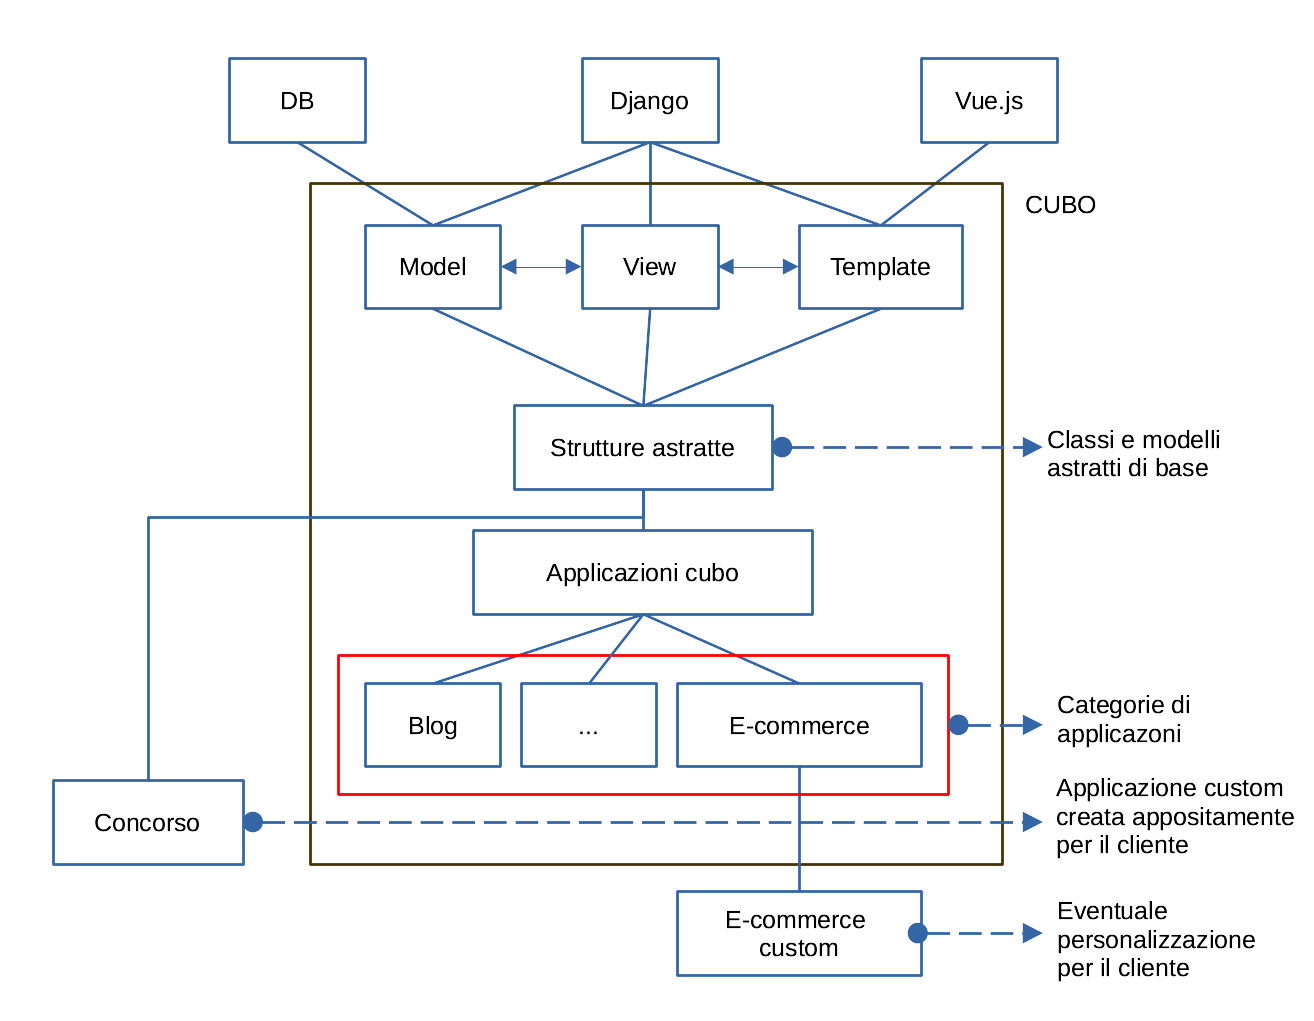
\includegraphics[width=1\linewidth]{cubo_scheme.png}
    \caption{Schema di Cubo}
\end{figure}

\subsubsection{DB, Django, Vue.js --- MVT}
Come anticipato nei capitoli precedenti Cubo è basato su Django, che rende possibile la creazione e comunicazioni tra le tre parti principali: Modello, Vista e Template.

Il \textbf{modello} comunica direttamente con il server di database, che tramite il dbms postgreSQL crea le tabelle, relazioni e vincoli definiti nei modelli.

La \textbf{vista} è una funzione che viene invocata quando l’utente apre una qualsiasi pagina sul sito web, gesisce la richiesta del client, spesso interrogando il database, e  restituisce tutte i dati necessari per strutturare correttamente ed in modo completo la pagina web.

La funzione dei \textbf{template} è quella di trasformare le informazioni logiche in elementi di markup html.
% Come si può notare dall’immagine xxx i dettagli del post (immagine, titolo, e sottotitolo) non sono hard-coded ma sono ricavate dalle variabili recuperate dalla vista.
I template sono semplici file html, con una sintassi adattata per le variabili di Django; è inoltre possibile eseguire funzioni direttamente all’interno del codice in caso di necessità.

Quando viene effettuata una richiesta, il server di django effettua tutte le operazioni attraverso le viste e restituisce all’utente una pagina html pura senza variabili o dati sensibili. Questo perché, a differenza di altri framework, django effettua un server-side rendering: il server effettua tutte le operazioni necessarie, e poi restituisce al browser client solamente il codice html.
Altri framework, come React o Vue.js, basati su javascript, effettuano invece tutte le operazioni a livello client attraverso il browser, dinamicizzando così il sito web.

Entrambe le opzioni sono valide, la scelta dipende dal contesto:
\begin{itemize}
    \item \textbf{server-side} rendering: gode di migliori performance, di sicurezza dei dati, ma le pagine web rimangono statiche;
    \item \textbf{client-side} rendering: gode di peggiori performance (variabili in base a prestazioni del dispositivo e scelta del browser), ma lavorando con javascript, si riesce a rendere le pagine dinamiche senza ricaricarle.
\end{itemize}
Scegliere una delle due soluzioni non esclude l’altra, ma è possibile combinarle per costruire una struttura \textbf{sicura} attraverso l’isolamento dei dati tramite server-side e \textbf{dinamica} tramite client-side. Per questo, per Cubo si adotta l’innesto di script Vue.js nei template django html.

\subsubsection{Modelli astratti}
Con modelli astratti si intende la creazione di classi standard (o estensione di classi Django), estendibili ed adattabili a molteplici situazioni. Per esempio, la classe astratta \textit{StandardPageMetaModel} è utilizzata come classe padre per ogni modello sul database, dato che racchiude al suo interno attributi di base comuni ad ogni modello, come titolo, sottotitolo, data di creazione/modifica, slug, immagine.

Oltre ai modelli astratti dentro a Cubo sono state implementate molteplici classi astratte, che spaziano dai form alle tabelle alle viste, e attraverso il principio dell'ereditarietà si riesce a riciclare le stesse righe di codice per diversi modelli e applicazioni. Per esempio la classe \textit{BaseCreate} è la classe padre per ogni vista comprensiva di un form (form-view) ed estende tre classi di django \textit{StaffuserRequiredMixin}, \textit{SuccessMessageMixin} e \textit{CreateView}, che permettono la creazione di una form-view ed effettuare i controlli sui permessi di amministratore e la validazione del form.
\begin{verbatim}
    class BaseCreate(StaffuserRequiredMixin,
                     SuccessMessageMixin, CreateView)
\end{verbatim}

Oltre a \textit{BaseCreate}, vengono riportate per completezza anche le altre classi \textit{Base} che si riferiscono ai form-view a livello amministratore, che attraverso il nome si autodescrivono.

\begin{verbatim}
    BaseCreate, BaseUpdate, BaseDelete, BaseIndex,
    BaseIsFeatured, BaseIsReady, BaseRank.
\end{verbatim}

\textit{BaseCreate} (e tutte le altre appena elencate) è una classe astratta e per renderla concreta è necessario estenderla in un caso reale: per la creazione di una form-view per il modello \textit{Post} presente nell'applicazione \textit{Blog}, è necessario estendere la classe \textit{BaseCreate} e sovrascrivere gli attributi specifici della classe nel caso d'uso (modello, form, template e messaggio di corretta crezione). Nell'esempio riportato sotto si definisce la creazione di una classe per la creazione di un'istanza della classe \textit{Post}:
\begin{verbatim}
    class PostCreate(BaseCreate):
        model = Post
        form_class = PostForm
        template_name = "blog/admin/post_form.html"
        success_message = "%(title_it)s salvato
                           con successo."
\end{verbatim}

\subsubsection{Applicazioni Cubo}
Le applicazioni sono il cuore di Cubo. Contengono al loro interno le implementazioni reali delle classi astratte di Cubo discusse nella sezione precedente. Le applicazioni sono delle sotto-cartelle di cubo che racchiudono al loro interno modelli, viste, template e url specifici per l'applicazione, oltre ad ogni file necessario per il corretto funzionamento di essa. Per la creazione di un modello specifico è necessario estendere la classe \textit{StandardPageMetaModel} e dopodichè definire tutti gli attributi specifici per quel modello dell'applicazione. Per il modello \textbf{Post}, oltre agli attributi standard, si definiscono:
\begin{itemize}
    \item la categoria di un post;
    \item blocchi personalizzati (vengono discussi successivamente);
    \item articoli correlati;
    \item tag relativi al post;
    \item l'ordinamento per il fetch dal database e le etichette del modello.
\end{itemize}


\begin{verbatim}
    class Post(StandardPageMetaModel):
        category = models.ForeignKey(
            "PostCategory",
            on_delete=models.CASCADE,
            blank=True,
            null=True,
            db_index=True,
            verbose_name="categoria",
        )
        content = JSONField(default=list, blank=True)
        related_posts = models.ManyToManyField("self",
                        blank=True, verbose_name="articoli
                        correlati")
        tags = models.ManyToManyField("PostTag", blank=True)

        class Meta:
            ordering = ["-publish_date", "rank"]
            verbose_name = "articolo"
            verbose_name_plural = "articoli"
\end{verbatim}
Per ogni applicazione, oltre a definire i modelli estendendo il padre \textit{StandardPageMetaModel}, si creano anche i Form specifici a livello utente estendendo la classe \textit{BaseModelForm} che racchiude tutti gli attributi della \textit{StandardPageMetaModel} e una funzione di inizializzazione di base dei campi.

\begin{verbatim}
    class PostForm(BaseModelForm):
        class Meta:
            model = Post
            fields = BaseModelForm.Meta.fields +
                        ["category", "related_posts",
                         "content", "tags"]
            widgets = {"related_posts":
                         Select2MultipleWidget,
                       "tags": Select2MultipleWidget}
\end{verbatim}

Per quanto riguarda i template delle specifiche applicazioni, si applica, anche su di essi, il principio dell'ereditarietà (come nei modelli e nelle viste), perché ogni template estende il padre \textit{\_base.html}. Il template padre definisce la struttura base della pagina html comprensiva di tutte le sue parti. Questo template è suddiviso in blocchi per integrarsi meglio e senza ripetizione di codice una volta che viene esteso. Suddividere in blocchi un tempalte significa racchiudere suddividere la pagina porzioni di codice. Per esempio una pagina html è possibile inizialmente suddividerla in due blocchi: \textit{head} e \textit{body}. Il file \textit{\_base.html} prenderà quindi la struttura di:

\begin{Verbatim}[commandchars=\\\[\]]
_______________________________________________________
<html>
    <head>
        \verbatimbold[]
            <meta charset="utf-8">
            <meta http-equiv="X-UA-Compatible"
                  content="IE=edge">
            <meta name="viewport" ...
        \verbatimbold[]
    </head>

    <body>
        \verbatimbold[]
            <h1>Pagina padre</h1>
            <p>Lorem ipsum dolor sit amet, consectetur
            adipiscing elit, sed do eiusmod tempor
            incididunt ut labore et dolore magna aliqua
            </p>
        \verbatimbold[]
    </body>
</html>
_______________________________________________________
\end{Verbatim}
Per questo esempio si presuppone che ogni pagina abbia gli stessi tag nel tag \textit{head}.
In questo caso, per la "pagina figlio" che estende \textit{\_base.html} non è necessario riscrivere tutti i componenti html, ma solamente quelli diversi; dato che i tag head sono uguali per ogni pagina, nella pagina figlio, cambia solamente il blocco \textbf{body}. La pagina figlio ha quindi la seguente implementazione:

\begin{Verbatim}[commandchars=\\\[\]]
______________________________________________________
\verbatimbold[]

\verbatimbold[]
    <h1>Pagina figlio</h1>
    <p>Lorem ipsum dolor sit amet, consectetur
    adipiscing elit, sed do eiusmod tempor
    incididunt ut labore et dolore magna aliqua
    </p>
\verbatimbold[]
______________________________________________________
\end{Verbatim}
Grazie all'utilizzo dei blocchi è possibile quindi apportare modifiche al blocco \textit{head} nel file \textit{\_base.html} e vederle riflesse anche nella pagina \textit{post.html} senza dover modificare altro codice.
In questo esempio sono stati utilizzati solamente due blocchi (head e body), mentre in cubo ne son presenti \textbf{più di trenta}, che suddividono la pagina in piccole sezioni. La tecnica dell'ereditarietà dei template è estremamente utile ed utilizzata per la personalizzazione dei contenuti dei template figlio (come \textit{post.html}), ma mantentendo la scrittura del codice pulita e senza riscrivere lo stesso pezzo di codice in parti diverse del progetto.

\subsubsection{Personalizzazione per cliente}
Può capitare che lo stesso template soddisfi le esigenze di un cliente, ma non quelle di un altro, in questo caso django permette sovrascrittura dei file template in modo da poterlo strutturare diversamente senza sovrascrivere il file originale. Per comprendere al meglio questa parte è necessario definire come viene importato Cubo dentro ad ogni applicazione web.
Cubo è una libreria e viene installata come fosse un normalissimo pacchetto python. Per renderlo effettivamente parte del sito è necessario aggiungere le applicazioni Cubo che si desiderano nelle INSTALLED\_APPS del sito creato. Per esempio per un nuovo sito dal nome \textit{shop.unimore.it} si vuole utilizzare le applicazioni catalogo, e-commerce e carrello, per permettere al proprietario del sito di poter vendere i propri prodotti sul sito. Nella variable INSTALLED\_APPS si vanno ad aggiungere il nome delle applicazioni precedute dal nome del pacchetto (in questo caso Cubo) nel seguente modo:
\begin{Verbatim}
                INSTALLED_APPS = [
                    *INSTALLED_APPS,
                    "cubo.catalogue",
                    "cubo.shop",
                    "cubo.cart",
                ]
\end{Verbatim}
Una volta aggiunte le applicazioni desiderate alle INSTALLED\_APPS, queste diventano attive e funzionanti. Non è possibile modificare i modelli e le viste di Cubo, è però possibile sovrascrivere il template ricreando il path corretto. La sovrascrittura permette quindi di modificare la struttura del template per i clienti con esigenze speciali senza dover modificare i file originali in Cubo.

È possibile che la sola sovrascrittura non sia abbastanza per soddisfare tutte le esigenze, vengono quindi creati i \textit{tempaltetags}. I templatetags sono dei file python che vengono invocati dal template come fossero delle funzioni e possono interagire con i modelli e con il database come fossero delle Viste. Questo è fondamentale quando i dati che vengono forniti dalla Vista non sono adatti al "nuovo" template.
I tempaltetags vengono spesso utilizzati anche in Cubo quando più template necessitano dell'utilizzo delle stesse funzioni.

\subsubsection{Applicazioni ad-hoc}
Cubo è un cms completo che copre l'80\% circa delle richieste dei clienti, ma per il 20\% rimanente è necessario intervenire direttamente sul singolo sito web creando una o più applicazioni ad-hoc. Queste applicazioni custom vengono create a partire dai fondamenti di cubo discussi nelle sezioni precendenti (modelli e classi astratte) per avere una base di partenza comune e poter fare affidamento sulle strutture stabili.


\textbf{FACCIO UN ESEMPIO DI SITO CON APP CUSTOM CHE HO FATTO?}

\subsection{Workflow}
Il work-flow segue il paradigma MVT (Model-View-Template) precedentemente discusso.

Ogni modello del CUBO estende la classe \textit{StandardPageMetaModel} che racchiude al suo interno gli attributi di base comuni ad ogni sotto modello, (come titolo, sottotitolo, data di creazione, slug, immagine…).
Il modello \textit{Post} comprende, oltre agli attributi dello \textit{StandardPageMetaModel}, anche una categoria, il contenuto del post, i tag e i post correlati (si veda sezione 3.3.3).
Una volta creato il modello è necessario creare i file di migrazione per il database.
Le migrazioni sono il mezzo attraverso il quale i cambiamenti che vengono effettuati nei file dei modelli, vengono effettivamente riflessi anche nelle tabelle sul database.
Ogni volta effettuate le modifiche ai file dei modelli, è necessario generare anche i file di migrazione. Django include i comandi per autogenerare i file di migrazioni e per riflettere le modifiche sul database per rendere effettivi i  cambiamenti:
\begin{verbatim}
            python manage.py makemigrations
            python manage.py migrate
\end{verbatim}

\subsection{Pannello amministratore}
Una volta sviulppato il sito web, è necessario configurare gli opportuni parametri. Tutta l'impostazione del sito web parte dal pannello amministratore dove è possibile modificare le configurazioni del sito e delle varie applicazioni e caricare i contenuti che si andranno poi a visualizzare a livello utente.
\begin{figure}[H]
    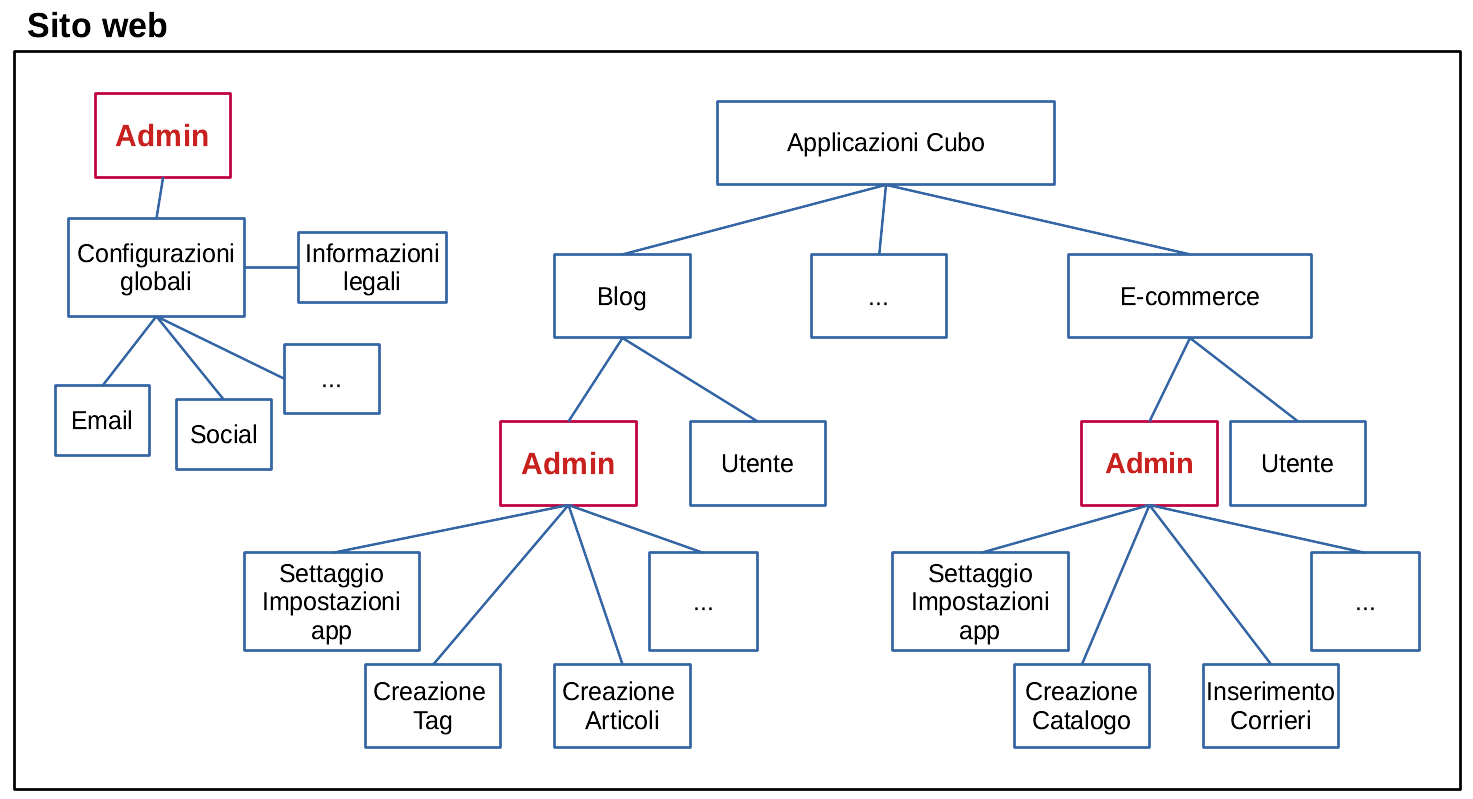
\includegraphics[width=1\linewidth]{admin.png}
    \caption{Schema di Cubo}
\end{figure}

Ogni applicazione dispone delle proprie modalità ed impostazioni di caricamento contenuti, in base alle esigenze ed alle necessità del caso d'utilizzo.

\subsubsection{Blocchi Cubo}
Come ogni cms che si rispetti, anche Cubo mette a disposizione dei "blocchi" prefabbricati per la costruzione di una pagina. I blocchi sono una libreria di elementi predefiniti che permettono di aggiungere contenuti, nelle varie pagine del sito, che l'amministratore crea dal pannello admin.

Esistono blocchi per gestire i seguenti tipi di componenti:
\begin{itemize}
    \item testo;
    \item immagini;
    \item galleria;
    \item documenti;
    \item video;
    \item citazioni;
    \item prodotto.
\end{itemize}
Ogni blocco è componibile con un altro in modo da lasciare libertà \break all'amministratore di rappresentare la pagina nel modo che ritiene migliore




























\clearpage
\section{Scelte tecnologiche}
In questa sezione si analizzano nel dettaglio le scelte tegnologiche che si adottano nel passagggio tra sviluppo e produzione di un'applicazione web.

\subsection{Server}

Una volta che l’applicazione web è stata sviluppata, è necessario assicurarsi che sia accessibile a tutti sul World Wide Web (WWW). Per fare ciò, ci sono tre principali alternative che andremo ad analizzare nel dettaglio elencandone inoltre, i vantaggi e gli svantaggi:
\begin{enumerate}
    \item acquistare un server fisico;
    \item acquistare un server in cloud;
    \item acquistare uno spazio gestito.
\end{enumerate}
1 --- con “acquistare un server fisico” si intende l’acquisto di tutti i componenti necessari per comporre un computer dedicato a uno o più siti web. Per questa soluzione sono necessarie diverse competenze:

\begin{itemize}
    \item essere aggiornati sui migliori componenti sul mercato;
    \item saper comporre un server;
    \item saper gestire un server, a partire dall’installazione del sistema operativo;
    \item saper gestire la sicurezza delle connessioni;
    \item saper gestire i database;
    \item saper gestire i backup;
    \item saper gestire gli aggiornamenti software;
    \item saper gestire i malfunzionamenti hardware-software;
\end{itemize}

Come si può notare dall’elenco delle competenze, sono necessari uno o più sistemisti che si dedichino alla gestione del server, e di tutto ciò che gli gira intorno.
Scegliere questa alternativa implica avere la responsabilità completa della gestione del server dalla propria parte, ma anche che nessun altro avrà i permessi di accedere ai dati (se la sicurezza è adeguata), e che la privacy dell’intero ecosistema è garantita. Uno svantaggio da tenere in considerazione con questa opzione è che i componenti non durano per sempre, possono danneggiarsi, guastarsi, e vanno quindi sostituiti con dei componenti nuovi, inoltre per garantire la privacy come detto precedentemente, è necessario gestire accuratamente la sicurezza.

2 --- con “acquistare un server in cloud” si intende l’utilizzo di una IAAS (infrastructure as a service). A differenza della soluzione precedente, questa opzione risparmia tre passaggi fondamentali del setup di un server: acquisto componenti, composizione server e installazione sistema operativo.
Questa soluzione è perfetta per chi vuole la completa autonomia sul proprio server, in modo da poter gestire applicazioni complesse, ma allo stesso tempo non deve tener conto degli svantaggi dell’opzione precedente. Le performance dei server sono garantite dal provider del servizio che curerà l’obsolescenza dei componenti e la loro costante manutenzione. Il provider inoltre si fa carico di alcuni livelli di sicurezza per l’accesso alle risorse. Esempi di aziende che offrono queste infrastrutture sono Digitalocean, Amazon Lightsail, Google cloud platform o Microsoft Azure.

3 –-- con “acquistare uno spazio gestito” si intende l’utilizzo di una PAAS (platform as a service). Questa soluzione permette allo sviluppatore di concentrarsi unicamente sullo sviluppo di applicazioni migliori, senza investire tempo nella preparazione e manutenzione del server e del software di gestione, che sarà completamente a carico del provider della piattaforma.
Il modello di piattaforma più diffuso negli ultimi anni è sicuramente Docker, una tecnologia di containerizzazione che consente la creazione e l'utilizzo dei container Linux.
Un container Linux è un insieme di uno o più processi isolati dal resto del sistema. Poiché tutti i file necessari per eseguire tali processi vengono forniti da un'immagine distinta, i container Linux sono portabili e coerenti in tutti gli ambienti, dallo sviluppo, ai test, fino alla produzione. Questo li rende molto più veloci rispetto ai tradizionali flussi di sviluppo che dipendono dalla replica degli ambienti di test tradizionali. I container, oltre a godere di una grandissima popolarità e ad essere apprezzati per la loro facilità d'uso, hanno un ruolo importante anche nella sicurezza IT, poiché la compromissione di un singolo container non va ad influire sull’intero sistema.
Docker considera i container come macchine virtuali modulari estremamente leggere, offrendo la flessibilità di creare, distribuire, copiare e spostare i container da un ambiente all'altro, ottimizzando così le app per il cloud.

Come si può notare dall’immagine sottostante, a differenza delle classiche macchine virtuali, i container linux condividono lo stesso sistema operativo, e risultano quindi molto più performanti, motivo principale della loro diffusione.

Studio Indaco ha deciso di optare per la terza categoria di deploy di un’applicazione web. In particolare vengono utilizzari due diversi servizi in base alle necessità di risorse e sviluppo del cliente: Heroku e fly.io.

\subsection{Database}
Con base di dati (o banca dati, a volte abbreviato con la sigla DB, dall'inglese database) in informatica si indica un insieme di dati strutturati ovvero omogeneo per contenuti e formato, memorizzati in un computer. Questi rappresentano di fatto la versione digitale di un archivio dati o schedario.
Le informazioni contenute in una banca dati sono strutturate e collegate tra loro secondo un particolare modello logico scelto dal progettista, tra relazionale, gerarchico, reticolare o a oggetti. Gli utenti si interfacciano con i databae dati attraverso i cosiddetti linguaggi di interrogazione come ad esempio SQL e grazie a particolari applicazioni software dedicati, come il DBMS (database management system).

SQL ()……….

Un DBMS è un software che si frappone fra l’utente ed i dati veri e propri. Grazie a questo strato intermedio l’utente e le applicazioni non accedono ai dati così come sono memorizzati effettivamente, cioè alla loro rappresentazione fisica, ma ne vedono solamente una rappresentazione logica. Ciò permette un elevato grado di indipendenza fra le applicazioni e la memorizzazione fisica dei dati. L’amministratore del database, se ne sente la necessità, può decidere di memorizzare i dati in maniera differente o anche di cambiare il DBMS senza che le applicazioni, e quindi gli utenti, ne risentano. La cosa importante è che non venga cambiata la rappresentazione logica di quei dati, che è la sola cosa che i loro utilizzatori conoscono. Questa rappresentazione logica viene chiamata ‘schema del database’ ed è la forma di rappresentazione dei dati più a basso livello a cui un utente del database può accedere.

Esistono svariati DBMS con caratteristiche e casi d’uso molto differenti, ma si possono classificare in due categorie principali: ‘SQL’ e ‘NO SQL’.

SQL (Structured Query Language) che, come suggerisce il nome, è un linguaggio volto all’interrogazione di dati altamente strutturati in tabelle prima definite.
A differenza dei linguaggi NO SQL (Not Only SQL), che non hanno una struttura fissa, ma nascono dunque con l’idea di rappresentare dati eterogenei tra di loro e che non hanno sempre gli stessi attributi.

I DBMS NO SQL sono in genere più veloci rispetto alla loro controparte, ma non sempre sono adatti ad ogni caso d’uso. È preferibile utilizzare un database SQL quando si andranno ad interrogare i DBMS con query complesse ed a lavorare con tipi di dati in relazione tra di loro; è invece preferibile l’utilizzo di un database NO SQL quando si necessita di più flessibilità nei dati e le query sono realtivamente semplici.
Come con la dura scelta del server, lo sviluppatore/sistemista è chiamato a decidere anche dove posizionare il proprio database, se gestirlo autonomamente o acquistarne uno in cloud da un fornitore di servizi. Tra i più famosi fornitori di servizi troviamo Amazon AWS (dove Studio Indaco depone i propri database).


\end{document}